\documentclass[11pt,a4paper]{article}

\usepackage[margin=2.5cm]{geometry}
\usepackage{graphicx}
\usepackage{booktabs}
\usepackage{amsmath,amssymb}
\usepackage{xcolor}
\usepackage{enumitem}
\usepackage{caption}
\usepackage{hyperref}
\usepackage{fancyhdr}
\usepackage{titlesec}
\usepackage{float}

% --- Colours ---
\definecolor{accent}{HTML}{2d3436}

% --- Header/footer ---
\pagestyle{fancy}
\fancyhf{}
\rhead{\small Girish Narayanan}
\lhead{\small LCAS --- Weekly Report}
\rfoot{\small\thepage}
\renewcommand{\headrulewidth}{0.4pt}

% --- Experiment environment ---
\newcounter{expnum}
\newenvironment{experiment}[1]{%
  \refstepcounter{expnum}%
  \subsection*{Experiment \theexpnum: #1}%
  \vspace{-0.5em}%
}{\vspace{1em}}

\newcommand{\setup}[4]{%
  \noindent
  \begin{tabular}{@{}p{2.8cm}p{11cm}@{}}
    \toprule
    \textbf{Variables}    & #1 \\
    \textbf{Constraints}  & #2 \\
    \textbf{Residual}     & #3 \\
    \textbf{Solver}       & #4 \\
    \bottomrule
  \end{tabular}
  \vspace{0.8em}
}

% --- Section styling ---
\titleformat{\section}{\large\bfseries\color{accent}}{}{0em}{}[\vspace{-0.3em}\rule{\textwidth}{0.4pt}]

% --- Graphics path ---
\graphicspath{{assets/}{../../data/results/inversion_diagnostics/}}

\begin{document}

% ============================================================
% TITLE
% ============================================================
\begin{center}
  {\LARGE\bfseries Winding Ambiguity \& Specular Glint Analysis}\\[0.5em]
  {\large Weekly Report --- 13 March 2026}\\[0.3em]
  Girish Narayanan
\end{center}
\vspace{1em}

% ============================================================
\section{Context}

Test case: IS-901.\;
$\boldsymbol{\omega}_\text{true} = (0.5,\,-0.3,\,2.0)\,^\circ/\text{s}$,\;
$|\boldsymbol{\omega}_\text{true}| = 2.083\,^\circ/\text{s}$.

Experiments~1--4: 120\,s window, 100 observations, $\Delta t_\text{samp} \approx 1.21\,$s, $\sigma = 0.05$\,mag.\\
Experiments~5--6: 3600\,s window, 500 observations, peaks at indices 183, 260, 360.\\
Experiments~7--10: 3600\,s window, 500 observations. Exp~8 uses 30 random $(q_0, \boldsymbol{\omega}_0)$ pairs.

% ============================================================
\section{Experiments (Recap from 10 March)}

% --- Exp 1 ---
\begin{experiment}{Forward Propagation --- Analytic $\boldsymbol{\omega}$, Exact Attitude, Hi-fi}

\setup
  {None (no free parameters)}
  {IS-901; $q_{k-1}, q_k$ exact from true trajectory; orientation: arb160; hi-fi shadowing}
  {MSE between reconstructed and observed LC (computed, not optimised)}
  {None --- $\boldsymbol{\omega} = \mathrm{rotvec}(q_{k-1}^{-1}\, q_k) / \Delta t_\text{samp}$ (analytic); Euler forward propagation from $q_k$}

\textbf{Result:} Reconstructed LC overlays truth. At $\Delta t_\text{samp} \approx 1.21\,$s the rotation is $\sim$2.5$^\circ$---no winding ambiguity.

\begin{figure}[H]
  \centering
  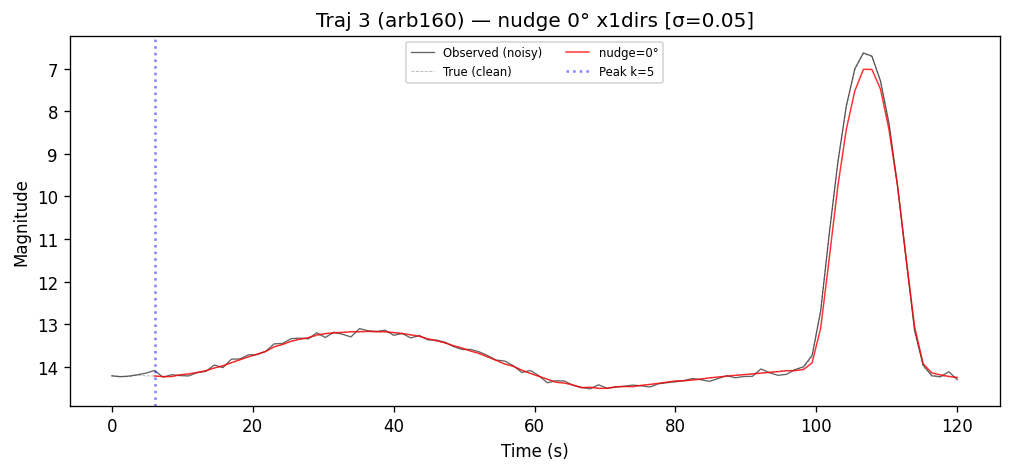
\includegraphics[width=0.82\textwidth]{micro01b_qnudge_2.08dps_traj3_nudge0.png}
  \caption{Hi-fi forward propagation from exact $q_k$ with analytic $\boldsymbol{\omega}$ (trajectory~3, arb160).}
\end{figure}

\end{experiment}

% --- Exp 2 ---
\begin{experiment}{Forward Propagation --- Analytic $\boldsymbol{\omega}$, 3$^\circ$ Attitude Nudge, Hi-fi}

\setup
  {Nudge direction (5 random unit vectors, seed 123; not optimised)}
  {Same analytic $\boldsymbol{\omega}$ as Exp~1; $q_k$ nudged $3^\circ$ before propagation; hi-fi}
  {MSE per direction (computed, not optimised)}
  {None --- same analytic $\boldsymbol{\omega}$; Euler forward propagation from nudged $q_k$}

\textbf{Result:} Anisotropic sensitivity. Near the glint, some directions shift the peak by $>$2\,mag; others are benign.

\begin{figure}[H]
  \centering
  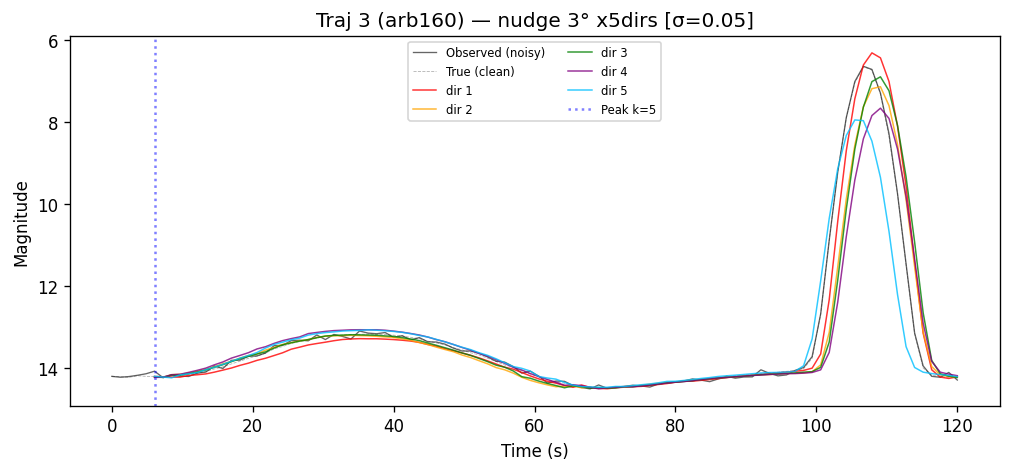
\includegraphics[width=0.82\textwidth]{micro01b_qnudge_2.08dps_traj3_nudge3.png}
  \caption{Hi-fi forward propagation from 3$^\circ$-nudged $q_k$ in 5 directions (trajectory~3, arb160).}
\end{figure}

\end{experiment}

% --- Exp 3 ---
\begin{experiment}{Forward Propagation --- Lo-fi Reconstruction, Exact Attitude}

\setup
  {None}
  {Same analytic $\boldsymbol{\omega}$ and exact $q_k$ as Exp~1; lo-fi reconstruction (no self-shadowing); observed LC is hi-fi; orientation: arb160}
  {MSE(lo-fi reconstruction, hi-fi observed)}
  {None --- forward evaluation only}

\textbf{Result:} Lo-fi phantom glint at $t \approx 60\,$s---facet in self-shadow produces false peak.

\begin{figure}[H]
  \centering
  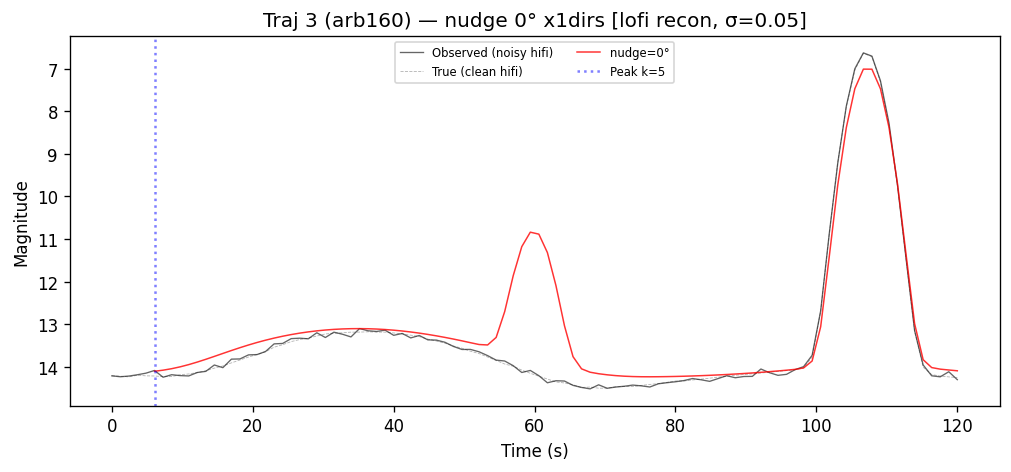
\includegraphics[width=0.82\textwidth]{micro01c_lofi_qnudge_2.08dps_traj3_nudge0.png}
  \caption{Lo-fi reconstruction vs hi-fi observed (trajectory~3, arb160). Phantom peak at $t \approx 60\,$s.}
\end{figure}

\end{experiment}

% --- Exp 4 ---
\begin{experiment}{Forward Propagation --- Lo-fi, Different Orientation}

\setup
  {Nudge direction (5 random unit vectors)}
  {Same analytic $\boldsymbol{\omega}$; $q_k$ nudged $3^\circ$; lo-fi reconstruction; orientation: $30^\circ$ about $\hat{x}$}
  {MSE(lo-fi, hi-fi) per direction}
  {None --- forward evaluation only}

\textbf{Result:} No phantom peak at this orientation. Lo-fi failure depends on active self-shadowing, unpredictable a priori.

\begin{figure}[H]
  \centering
  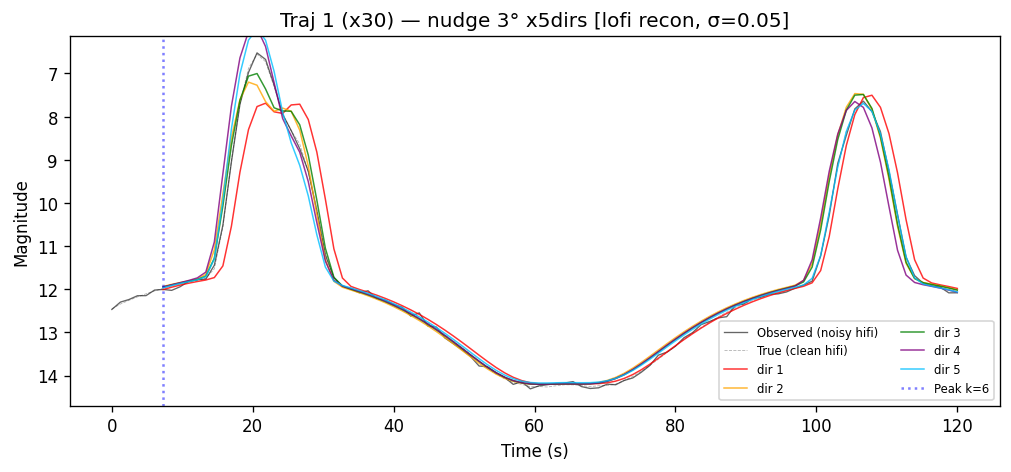
\includegraphics[width=0.82\textwidth]{micro01c_lofi_qnudge_2.08dps_traj1_nudge3.png}
  \caption{Lo-fi at benign orientation (trajectory~1, x30). No phantom peak.}
\end{figure}

\end{experiment}

\clearpage

% --- Exp 5 ---
\begin{experiment}{Staircase $\boldsymbol{\omega}$ Enumeration}

\setup
  {$\boldsymbol{\omega} \in \mathbb{R}^3$ (optimised per step)}
  {$q_A, q_B$ exact (oracle) at peaks 183, 260; $\Delta t = 555.5\,$s; soft lower barrier on $|\boldsymbol{\omega}|^2$ per step}
  {Objective: $1 - (q_\text{prop} \cdot q_B)^2 + \lambda_\text{barrier}$;\; post-hoc trough: $|b_\text{pred} - b_\text{ref}|$ (lo-fi, single epoch)}
  {L-BFGS-B, 8 sequential steps; axis-angle init step~0; $+2\pi/\Delta t$ increment subsequent steps}

\textbf{Result:} 8 winding solutions found. Trough scoring selects step~2 (wrong)---insufficient temporal leverage.

\begin{center}
\begin{tabular}{cccl}
  \toprule
  Step & $|\boldsymbol{\omega}|\;(^\circ/\text{s})$ & Arrival err & Trough err \\
  \midrule
  0 & 0.316 & 0.0 & 1.719 \\
  1 & 0.959 & 0.0 & 0.099 \\
  2 & 1.601 & 0.0 & 0.021 $\leftarrow$ best trough \\
  \textbf{3} & \textbf{2.230} & \textbf{0.0} & 0.792 $\leftarrow$ \textbf{true} \\
  4 & 2.883 & 0.036 & 0.044 \\
  5 & 3.509 & 0.0 & 0.134 \\
  6 & 4.180 & 0.0 & 1.749 \\
  7 & 4.824 & 0.0 & 1.491 \\
  \bottomrule
\end{tabular}
\end{center}

\end{experiment}

% --- Exp 6 ---
\begin{experiment}{Angular Momentum Conservation Filter --- Two-Leg Staircase}

\setup
  {$\boldsymbol{\omega} \in \mathbb{R}^3$ per leg per step}
  {$q_A, q_\text{mid}, q_B$ exact at peaks 183, 260, 360; leg~0 $\Delta t = 555.5\,$s; leg~1 $\Delta t = 721.4\,$s; lower + upper $|\boldsymbol{\omega}|$ barriers ($\pm 0.8\,\delta$)}
  {Per step: $1 - (q_\text{prop} \cdot q_\text{end})^2$ + barriers;\; L-filter: $\|\mathbf{L}_{\text{leg\,0}}[k] - \mathbf{L}_{\text{leg\,1}}[j]\|$}
  {L-BFGS-B per step; exhaustive $8 \times 8 = 64$ L-comparison at shared peak~260}

\textbf{Result:} Selected $(k{=}0,\, j{=}0)$. True: $(k{=}3,\, j{=}1)$. \textbf{Incorrect}---leg~1 staircase broken (near-$\pi$ singularity skips bands).

\begin{center}
\begin{tabular}{ccc}
  \toprule
  Step & Leg\,0 $|\boldsymbol{\omega}|\;(^\circ/\text{s})$ & Leg\,1 $|\boldsymbol{\omega}|\;(^\circ/\text{s})$ \\
  \midrule
  0 & 0.316 & 0.249 \\
  1 & 0.959 & 3.279 $\leftarrow$ gap \\
  2 & 1.601 & 3.509 \\
  3 & 2.230 & 3.995 \\
  \bottomrule
\end{tabular}
\end{center}

\end{experiment}

% ============================================================
\section{Decisions from 10 March}

\begin{itemize}[nosep]
  \item MIP ruled out (consulted Jack---insufficient discrete structure).
  \item Lo-fi scoring unreliable near glints (Exp~3--4).
  \item Single-trough scoring insufficient (Exp~5).
  \item L-conservation most promising $\omega$ filter, pending staircase fix.
\end{itemize}

% ============================================================
\clearpage
\section{New Experiments (This Week)}

% --- Exp 7 ---
\begin{experiment}{PAB Alignment Diagnostic at Brightness Peaks}

\setup
  {None (diagnostic---no free parameters)}
  {IS-901, standard test case; 500 epochs / 3600\,s; hi-fi with per-facet flux decomposition (\texttt{animate=True}); 3840 facets grouped into 14 unique normal directions (rounded to $4\,\text{dp}$); peaks detected via \texttt{argrelmin(mag, order=5)}}
  {$\hat{\mathbf{n}}_g \cdot \widehat{\text{PAB}}_\text{body}$ for each group $g$ at each epoch; fractional flux $= \Sigma f_g / \Sigma f_\text{total}$ per group at peaks}
  {None --- forward evaluation + decomposition}

\textbf{Result:} 43 peaks detected. At all 11 bright peaks (mag~$< 9$): a single normal group captures $>$77\% of total flux with $\hat{\mathbf{n}} \cdot \widehat{\text{PAB}} > 0.99$. Bright peaks are specular glints. Dim peaks (mag~$> 11$) are diffuse---dominated by bus broadside area, no near-perfect alignment.

\begin{figure}[H]
  \centering
  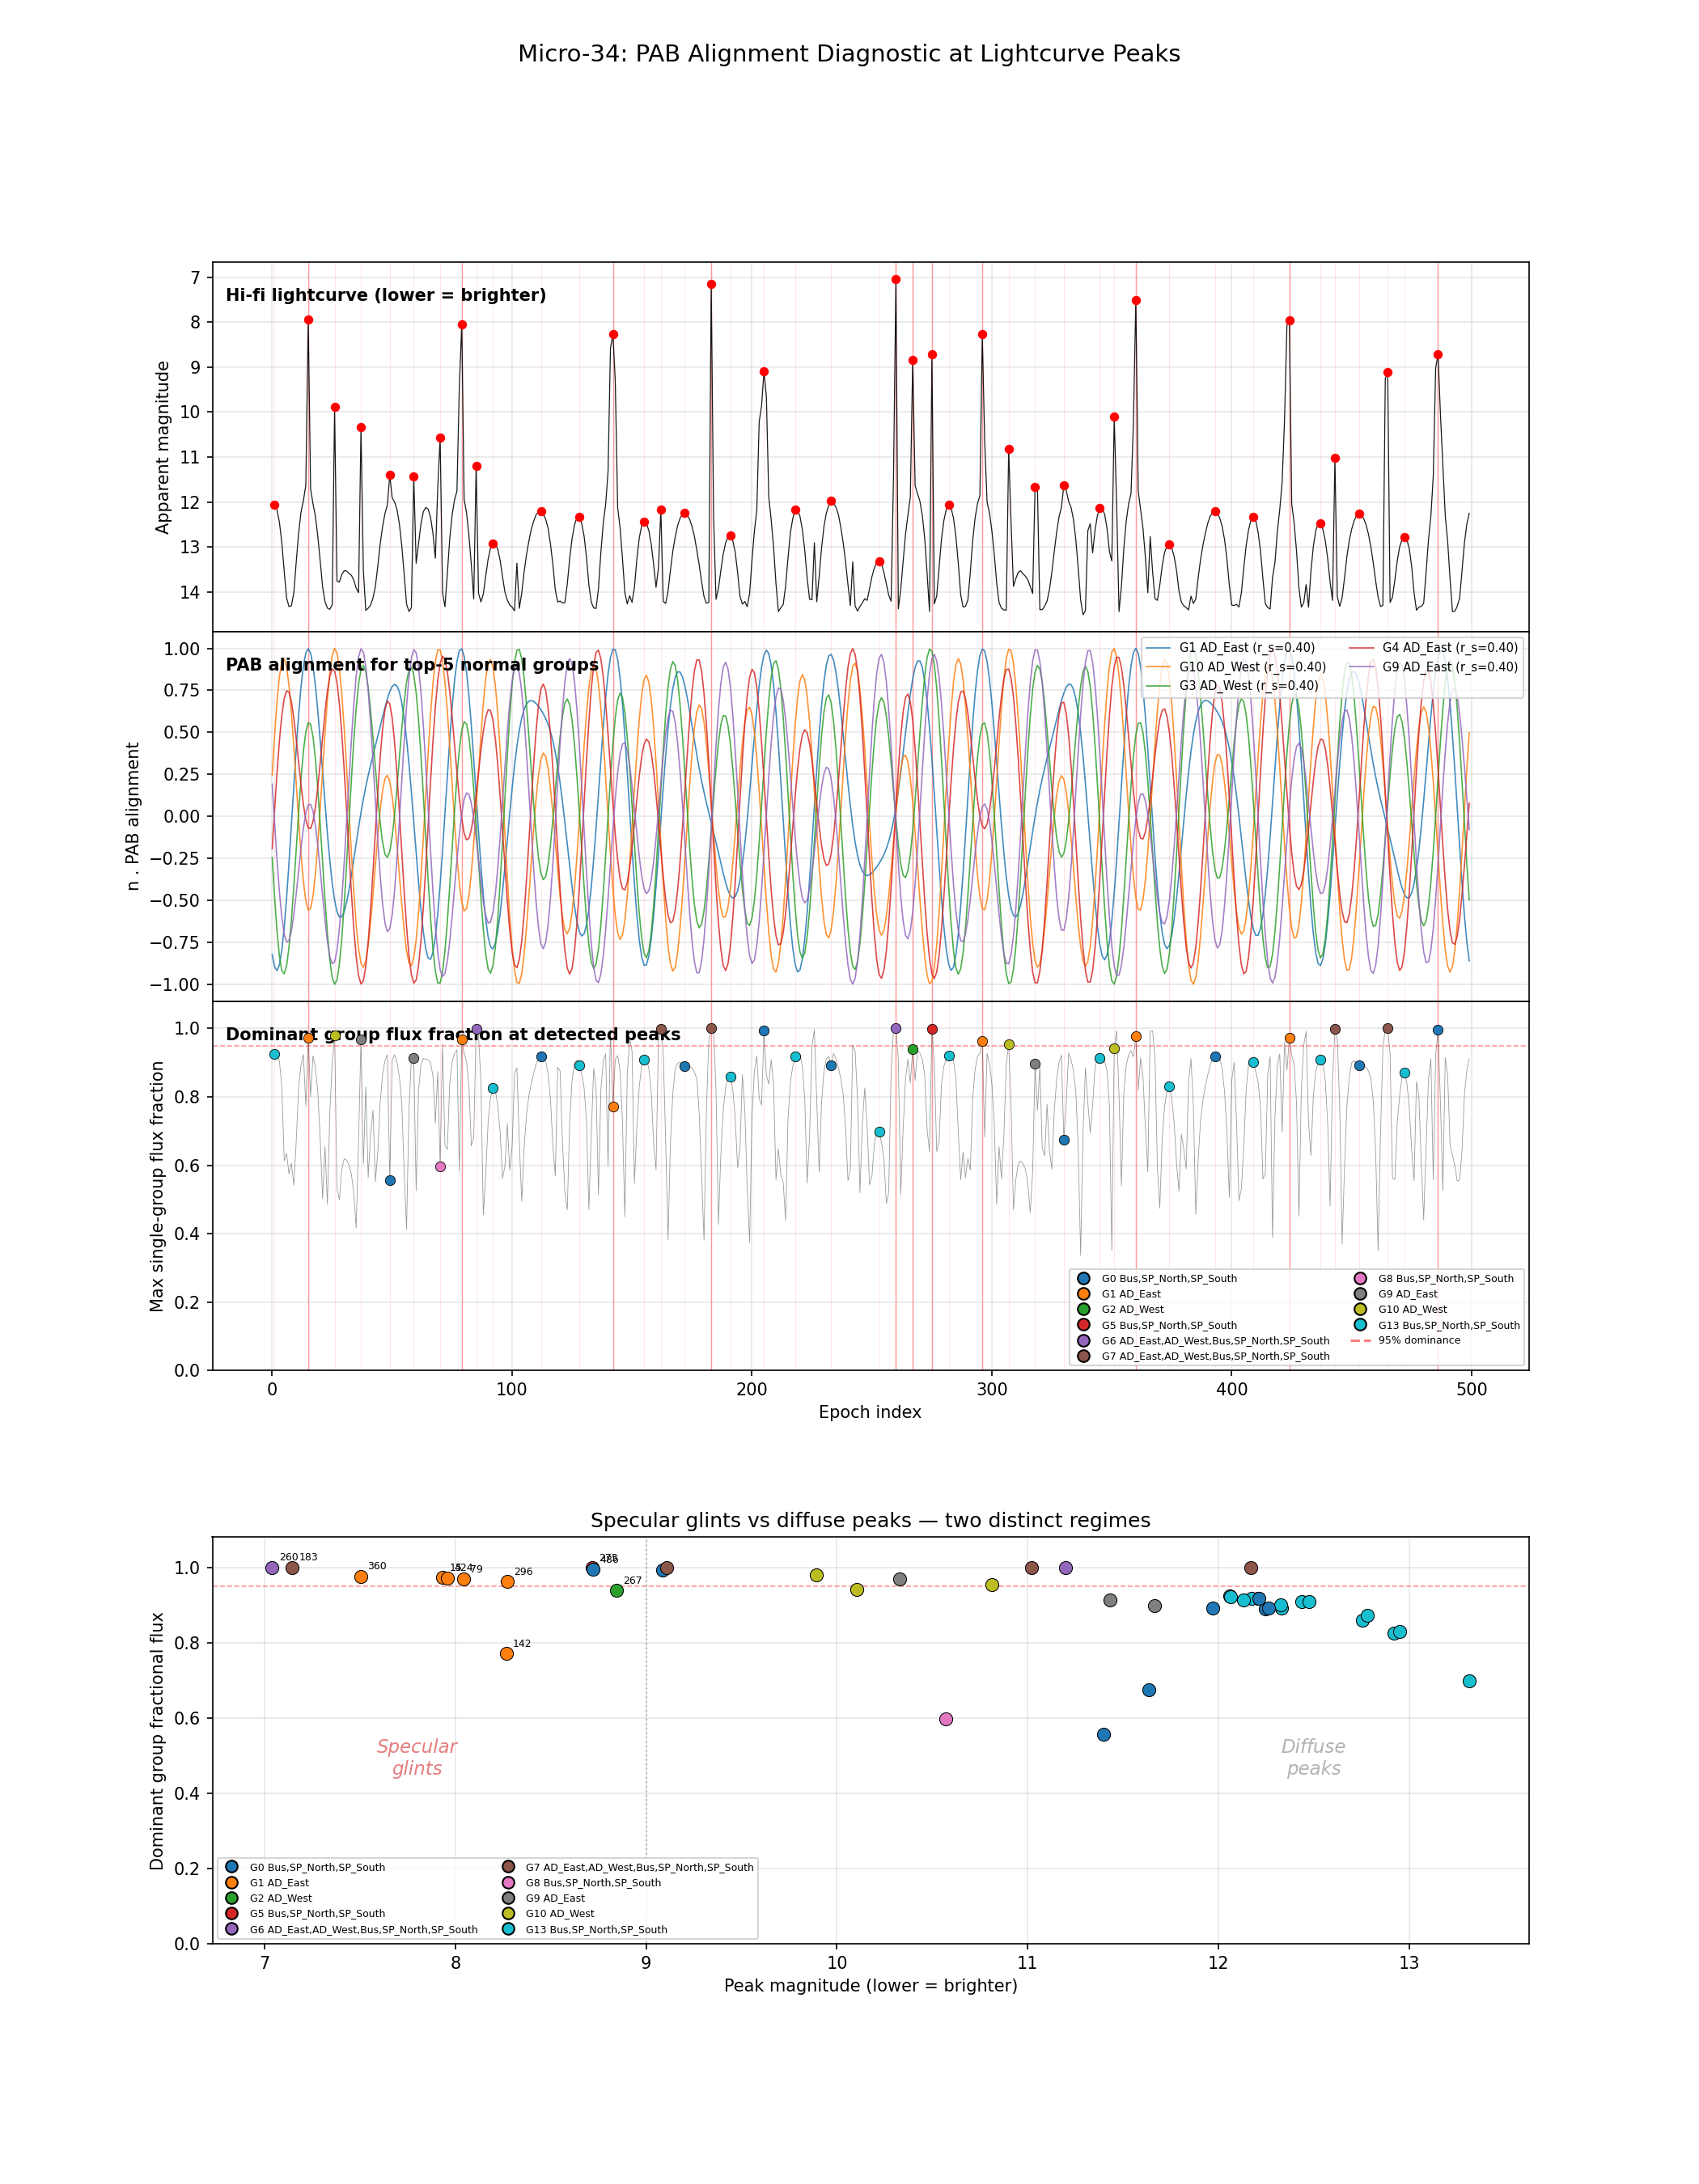
\includegraphics[width=\textwidth]{13_pab_alignment_diagnostic.png}
  \caption{micro34: 4-panel PAB diagnostic. Top: lightcurve. Second: $\hat{\mathbf{n}} \cdot \text{PAB}$ traces. Third: dominant-group flux fraction at peaks. Bottom: two-regime scatter (specular vs diffuse).}
\end{figure}

\end{experiment}

\clearpage

% --- Exp 8 ---
\begin{experiment}{Multi-Trajectory Glint Robustness (30 random trajectories)}

\setup
  {None (statistical survey)}
  {30 random $(q_0, \boldsymbol{\omega}_0)$ pairs; $q_0$ uniform on SO(3); $|\boldsymbol{\omega}|$ uniform in $[0.5,\,5.0]\,^\circ/\text{s}$; seeds 0--29; same IS-901 geometry/SPICE; hi-fi with per-facet flux; peaks via \texttt{argrelmin(order=5)}}
  {Per bright peak (mag~$< 9$): classified ``specular glint'' if dominant group frac $> 0.77$ and $\hat{\mathbf{n}} \cdot \text{PAB} > 0.99$; else ``near-miss''}
  {None --- forward evaluation per trajectory ($\sim$58\,s each, 29\,min total)}

\textbf{Result:}

\begin{center}
\begin{tabular}{lr}
  \toprule
  Total bright peaks (all 30 trajectories) & 439 \\
  Specular glints (strict) & 392 (89.3\%) \\
  Near-misses & 47 (10.7\%) \\
  Genuine counterexamples & 0 \\
  \bottomrule
\end{tabular}
\end{center}

All 47 near-misses have $\hat{\mathbf{n}} \cdot \text{PAB} > 0.984$ and $f > 0.54$---boundary cases, not violations. Near-miss rate increases with $|\boldsymbol{\omega}|$ (2\% at $<$1\,$^\circ$/s; 14\% at 3--5\,$^\circ$/s). Glint count $\approx 2.9\,|\boldsymbol{\omega}| + 6.3$ (linear).

\begin{figure}[H]
  \centering
  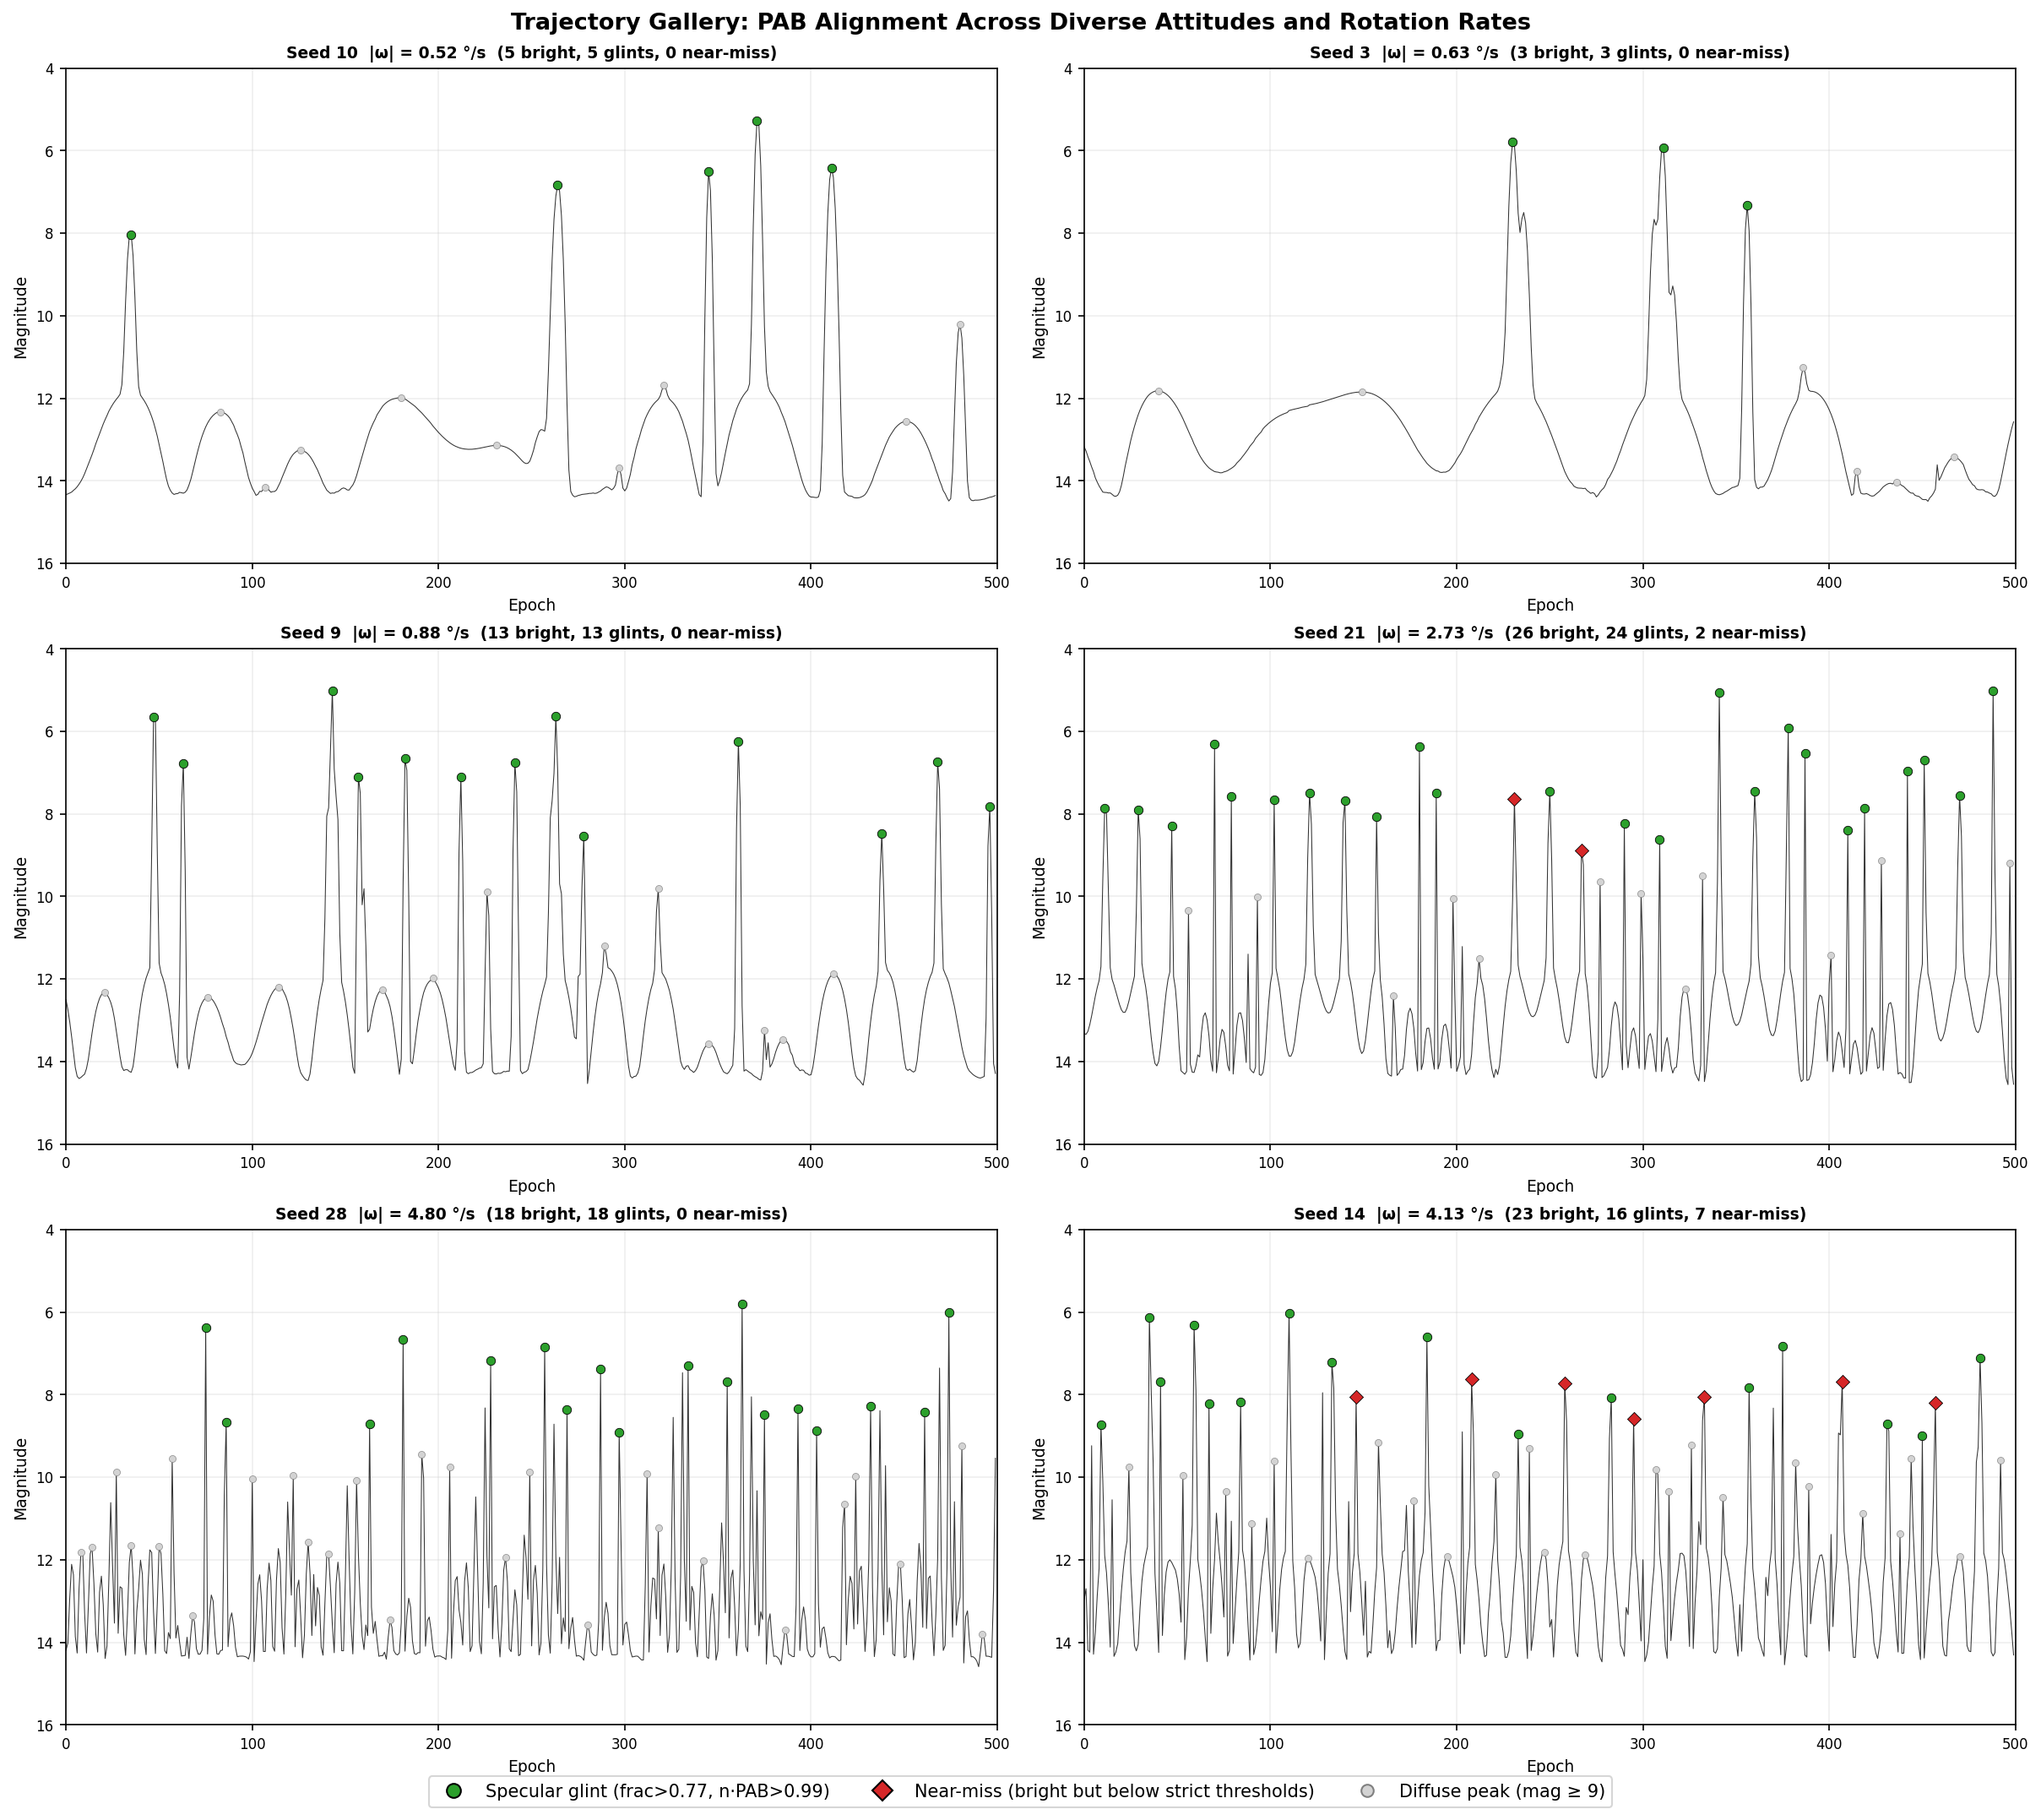
\includegraphics[width=\textwidth]{14_trajectory_gallery.png}
  \caption{micro35: 6 representative trajectories ($|\omega| = 0.52$--$4.80\,^\circ$/s). Green = specular glint, red = near-miss.}
\end{figure}

\begin{figure}[H]
  \centering
  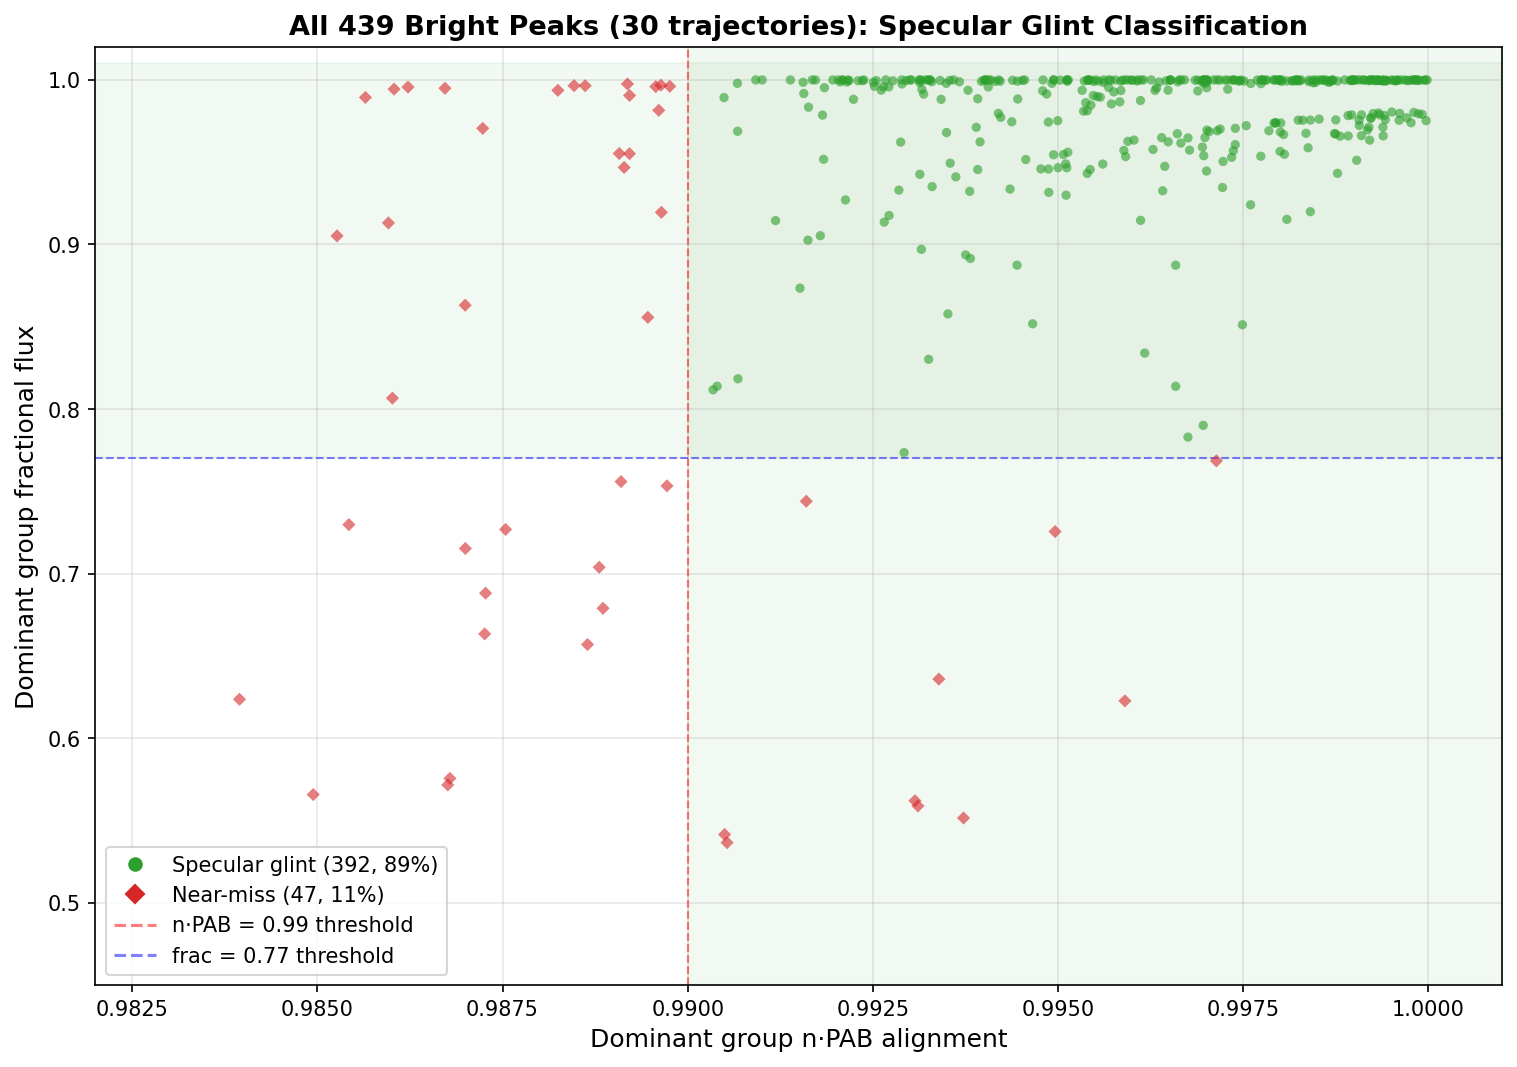
\includegraphics[width=0.82\textwidth]{16_bright_peak_scatter.png}
  \caption{micro35: All 439 bright peaks. Near-misses (red) cluster near the strict thresholds.}
\end{figure}

\end{experiment}

\clearpage

% --- Exp 9 ---
\begin{experiment}{PAB Alignment as Candidate Filter}

\setup
  {Angular threshold $\theta$ (swept 1$^\circ$--90$^\circ$)}
  {5643 iso-brightness candidates from micro10 at epoch~183 (glint, mag 7.15); 14 unique body-frame normals from IS-901; PAB$_\text{inertial}$ from SPICE; baseline: 5643 random SO(3) quaternions (seed 12345)}
  {Per candidate $q$: $\max_g\, \hat{\mathbf{n}}_g \cdot [R(q)\,\widehat{\text{PAB}}_\text{inertial}]$; candidate survives if $> \cos\theta$}
  {None --- vectorised dot products (no optimisation)}

\textbf{Result:}

\begin{center}
\begin{tabular}{ccccc}
  \toprule
  Threshold & Kill (iso) & Kill (random) & Iso survivors & Truth alignment \\
  \midrule
  $3^\circ$ & 100.0\% & 99.1\% & 0 & \\
  $5^\circ$ & 89.4\% & 97.6\% & 600 & $4.62^\circ$ $\checkmark$ \\
  $8^\circ$ & 0.0\% & 93.1\% & 5643 & \\
  \bottomrule
\end{tabular}
\end{center}

All 5643 iso-brightness candidates fall within $4.4$--$7.5^\circ$ of some normal. At $5^\circ$: 10$\times$ reduction while preserving truth. Key finding: iso-brightness matching at glint epochs \emph{implicitly} selects for PAB alignment---the two constraints are partially redundant.

\begin{figure}[H]
  \centering
  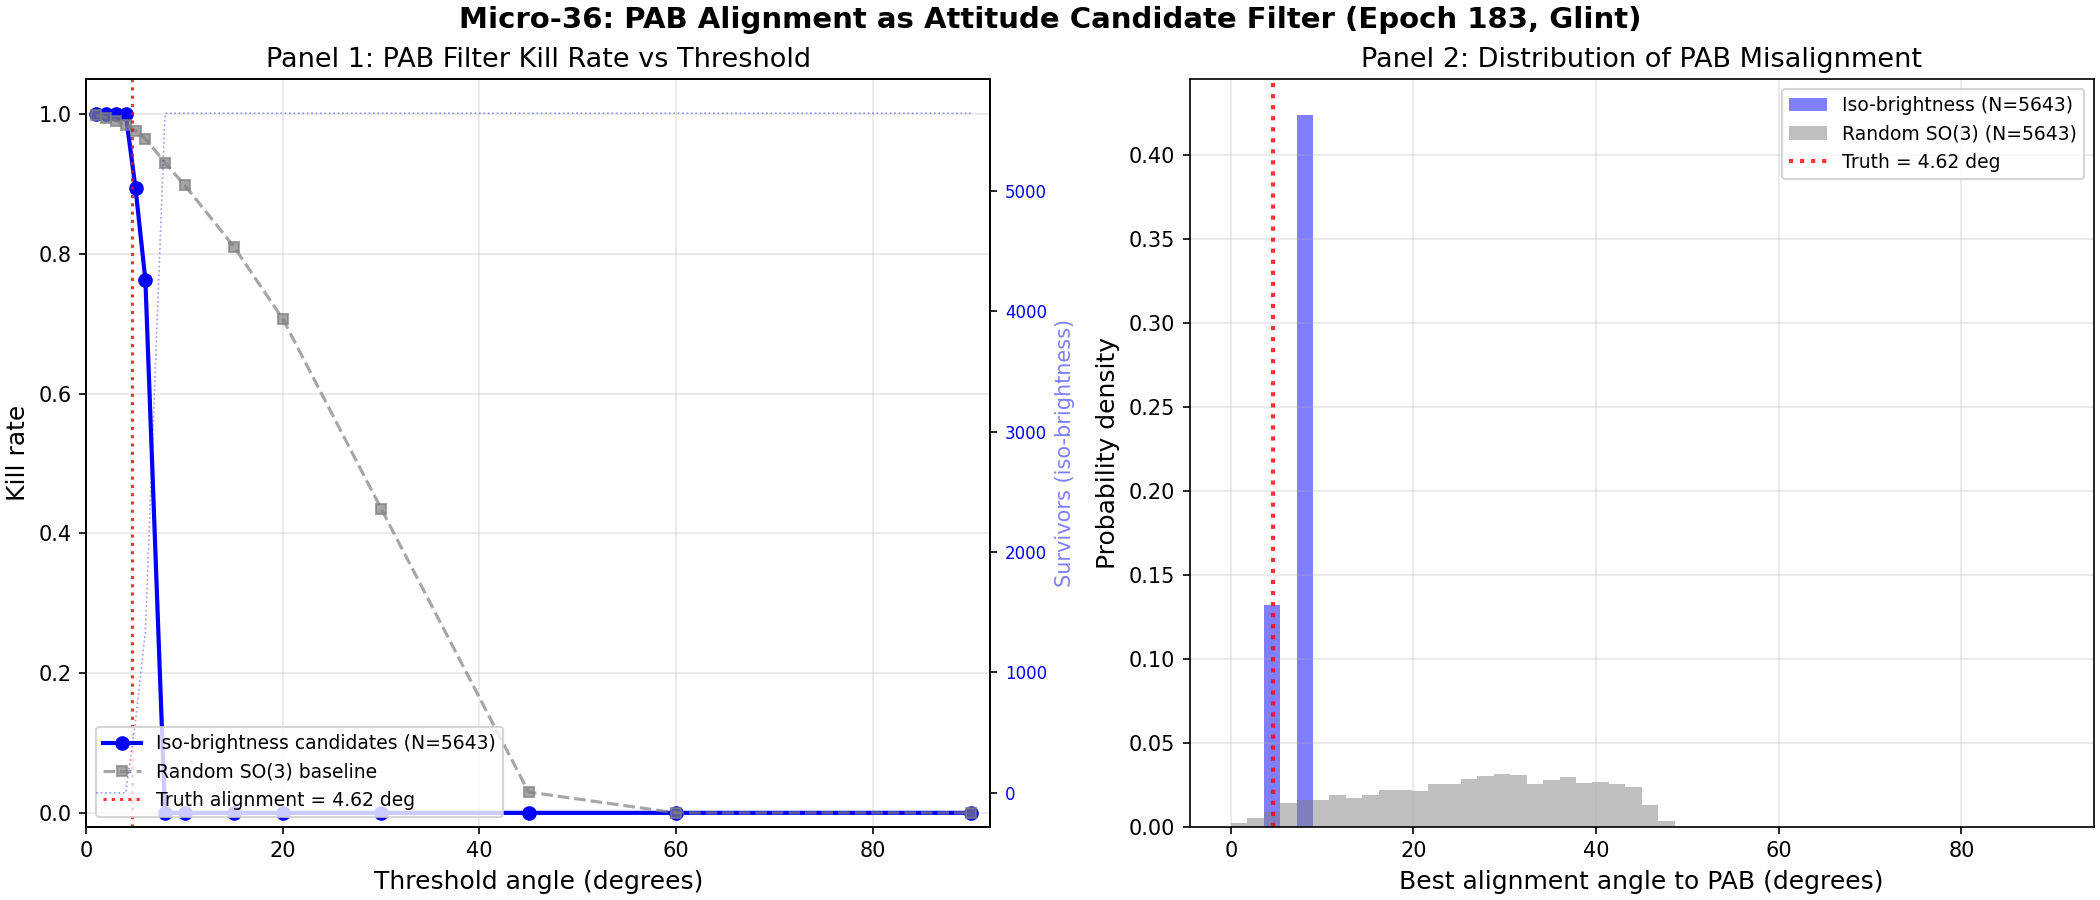
\includegraphics[width=\textwidth]{19_pab_candidate_filter.png}
  \caption{micro36: PAB alignment distributions. Iso-brightness candidates (blue) are already tightly clustered; random SO(3) (grey) spread across the full sphere.}
\end{figure}

\end{experiment}

% --- Exp 10 ---
\begin{experiment}{BRDF Specular Glint Profile Characterisation}

\setup
  {Misalignment angle $\theta$ (0--30$^\circ$, 0.1$^\circ$ steps); swept parameters: $n_\text{phong} \in \{50, 100, 200, 300, 500, 1000\}$; $r_s \in \{0.05, 0.10, 0.20, 0.40, 0.60, 0.80\}$; phase angle $\in \{5, 10, 20, 30, 45, 60\}^\circ$}
  {Synthetic flat plate, $1\,\text{m}^2$, GEO distance (36\,000\,km); Ashikhmin--Shirley BRDF; $\hat{\mathbf{k}}_1, \hat{\mathbf{k}}_2$ symmetric about PAB at half-angle $= \phi/2$; facet normal swept through PAB}
  {Apparent magnitude vs misalignment angle; FWHM of flux peak; specular $=$ diffuse crossing angle}
  {None --- pure BRDF evaluation (no satellite, no SPICE)}

\textbf{Result:}

\begin{center}
\begin{tabular}{cccc}
  \toprule
  $n_\text{phong}$ & FWHM ($^\circ$) & Spec $=$ Diff ($^\circ$) & Peak mag ($1\,\text{m}^2$) \\
  \midrule
  50 & 19.4 & 18.2 & 10.06 \\
  200 & 9.5 & 11.3 & 8.56 \\
  500 & 6.0 & 7.1 & 7.56 \\
  1000 & 4.3 & 6.0 & 6.81 \\
  \bottomrule
\end{tabular}
\end{center}

$n_\text{phong}$ controls lobe width (FWHM $\propto 1/\sqrt{n_\text{phong}}$). $r_s$ controls amplitude ($\sim$4\,mag range) but barely affects width. Phase angle is irrelevant ($< 0.01\,$mag variation across 5--60$^\circ$). Area scales linearly (verified exactly).

For IS-901 ($n_\text{phong} = 200$--$267$): specular-dominated region extends to $\sim$10$^\circ$.

\begin{figure}[H]
  \centering
  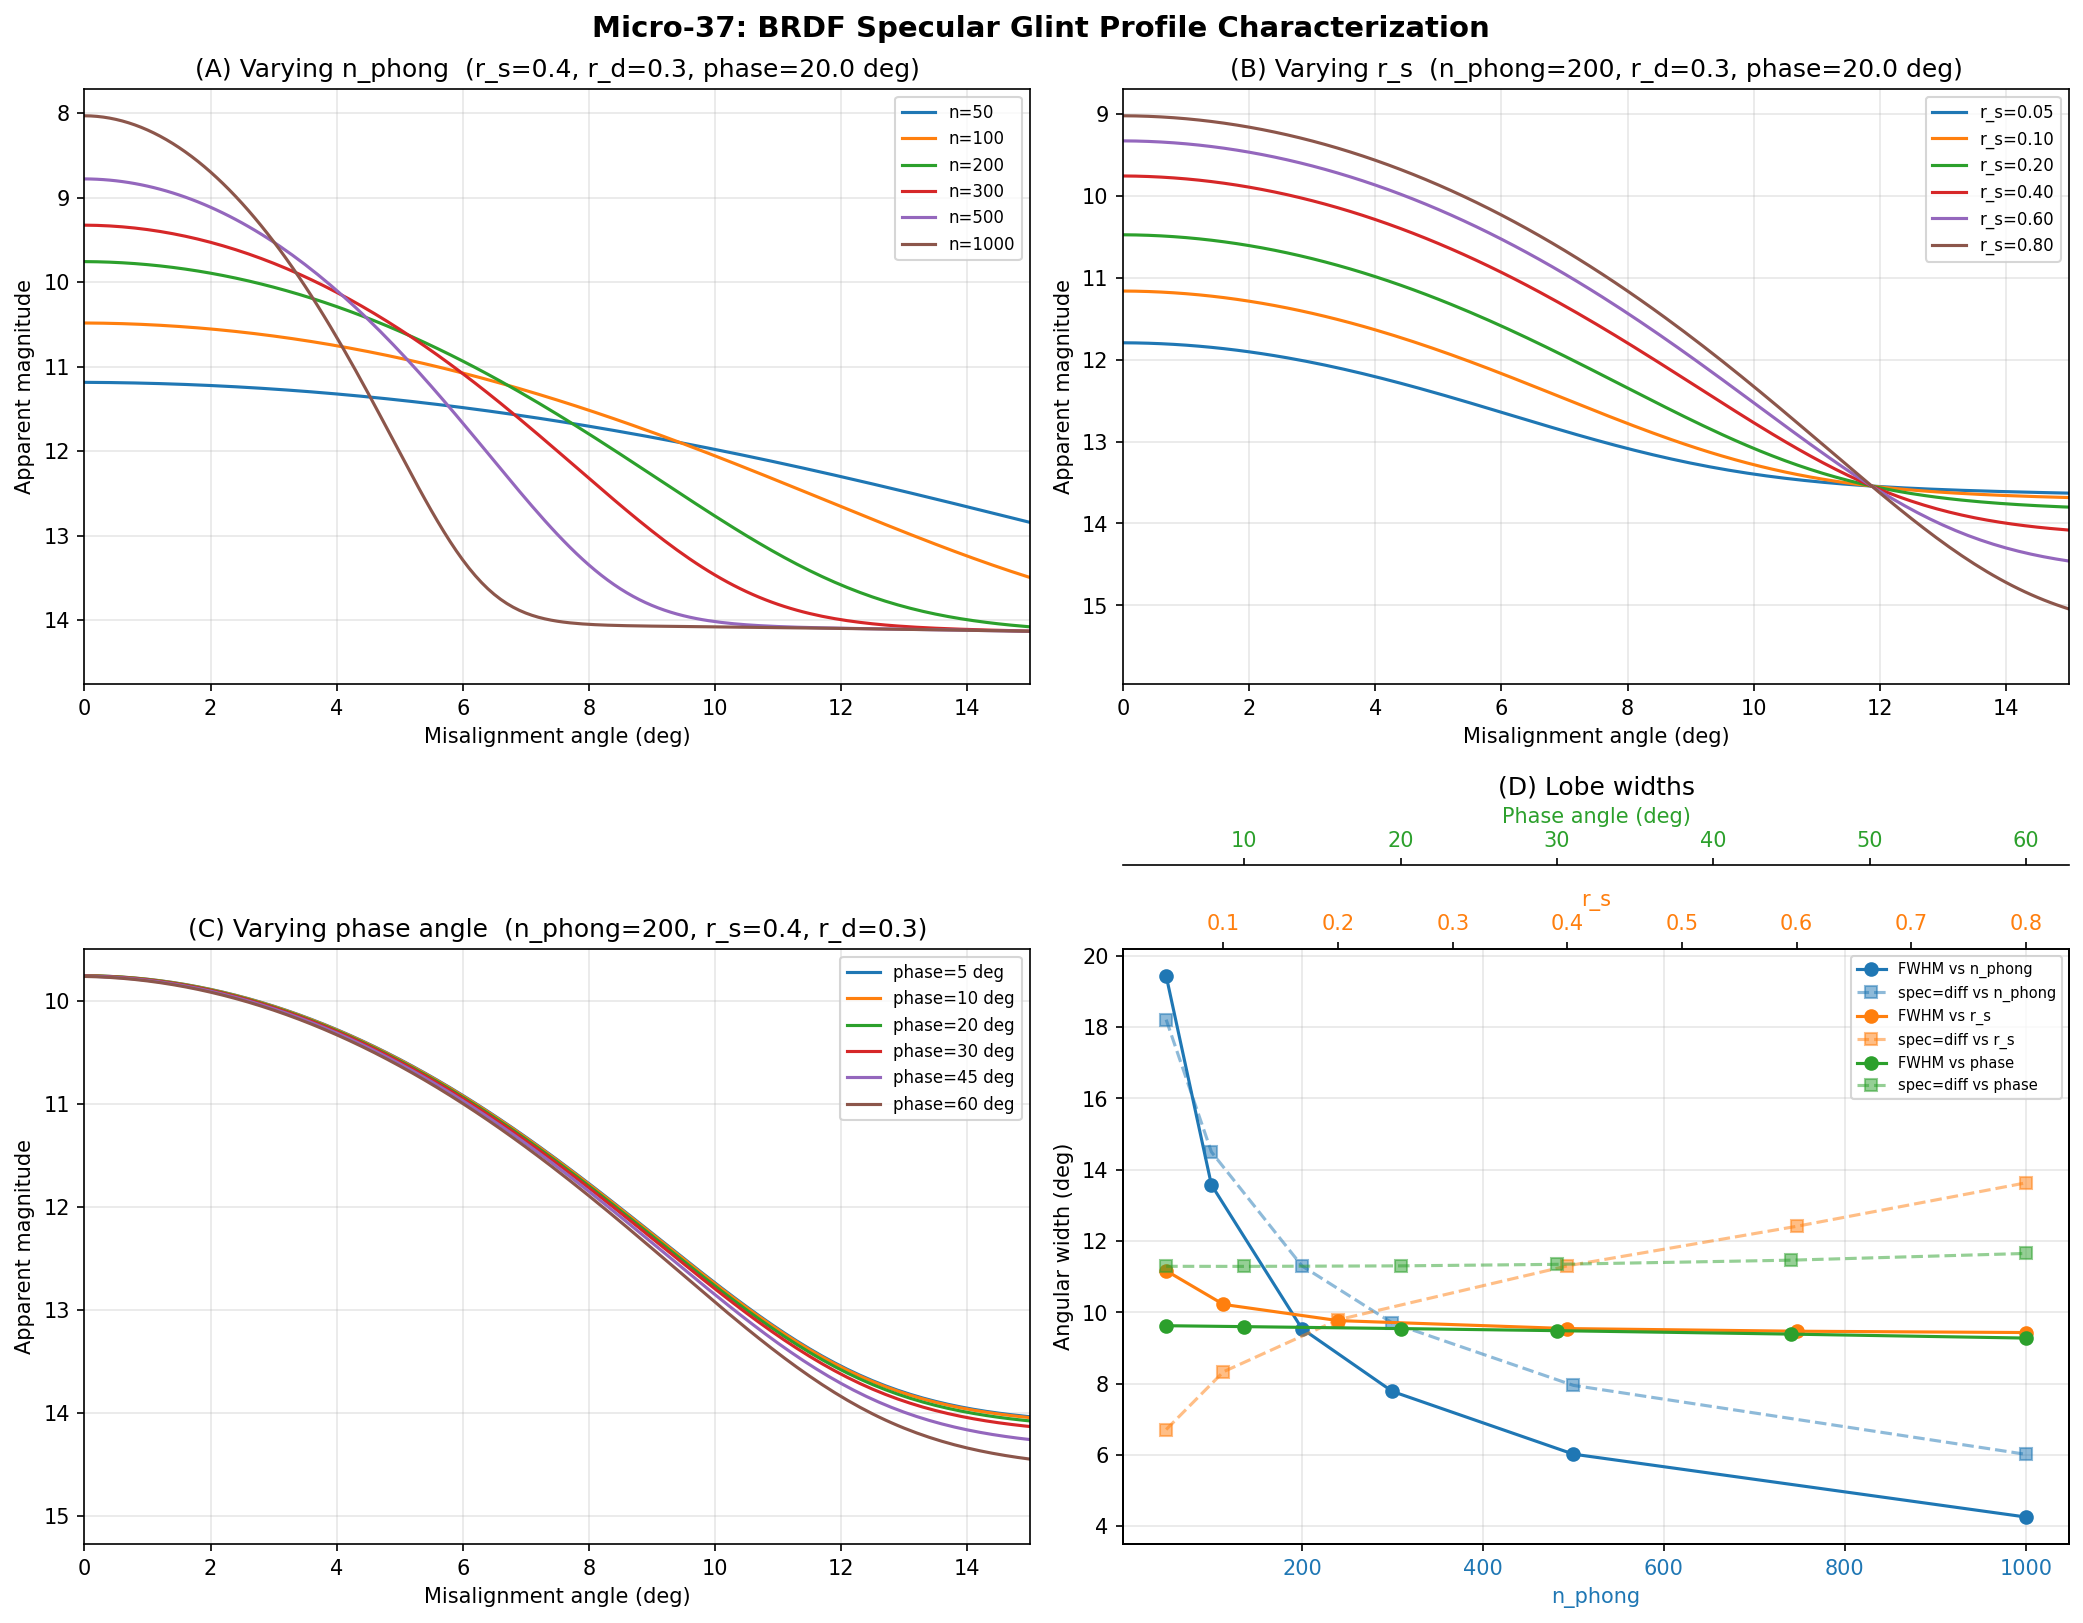
\includegraphics[width=\textwidth]{20_brdf_glint_profile.png}
  \caption{micro37: BRDF profile. (A)~$n_\text{phong}$ controls width. (B)~$r_s$ controls amplitude. (C)~Phase angle irrelevant. (D)~Lobe width summary.}
\end{figure}

\end{experiment}

% ============================================================
\section{Decisions}

\begin{itemize}[nosep]
  \item Bright peaks are specular glints (single-facet, $\hat{\mathbf{n}} \cdot \text{PAB} > 0.99$). Universal across 30 trajectories.
  \item PAB filter gives 10$\times$ candidate reduction at $5^\circ$ threshold, but is partially redundant with iso-brightness matching at glint epochs.
  \item Specular lobe width ($\sim$9.5$^\circ$ for IS-901) sets the angular scale for all alignment-based constraints.
  \item Phase angle has negligible effect on glint profiles---intrinsic material property.
\end{itemize}

% ============================================================
\section{Next Steps}

\begin{enumerate}[nosep]
  \item Component identification from glint properties (brightness, duration, recurrence).
  \item Multi-glint intersection: two glints from different normals $\to$ discrete $(q, \boldsymbol{\omega})$ candidates.
  \item Glint-based candidate generation: enumerate PAB circle analytically per normal, replace iso-brightness sampling.
  \item End-to-end pipeline test with non-oracle attitude candidates from iso-brightness stage.
\end{enumerate}

\end{document}
